\documentclass[conference]{IEEEtran}
\usepackage{cite}
\usepackage{amsmath,amssymb,amsfonts}
\usepackage{algorithm}
\usepackage{algpseudocode}
\usepackage{graphicx}
\usepackage{xcolor}
\usepackage{booktabs}
\usepackage{tikz}
\usetikzlibrary{arrows.meta,backgrounds,fit}
\usepackage{pgfplots}
\pgfplotsset{compat=1.18}
\usepackage{url}
\usepackage[hidelinks]{hyperref}

\newtheorem{proposition}{Proposition}
\newif\ifplaceholders
\placeholderstrue
\input{results_macros}

\definecolor{cBlue}{RGB}{52,101,164}
\definecolor{cRed}{RGB}{196,78,82}
\definecolor{cGreen}{RGB}{85,153,96}
\definecolor{cOrange}{RGB}{221,132,52}
\definecolor{cPurple}{RGB}{129,114,179}
\definecolor{cGray}{RGB}{120,120,120}
\tikzset{box/.style={draw=#1!70!black,fill=#1!12,rounded corners=3pt,align=center,font=\footnotesize,minimum height=1.05cm,text width=2.85cm,line width=0.6pt},box/.default=cBlue,arr/.style={-{Stealth[length=2.2mm]},line width=0.6pt,draw=black!75},darr/.style={arr,dashed}}
\pgfplotsset{every axis/.append style={font=\footnotesize,grid=major,grid style={gray!25},legend style={font=\scriptsize,draw=gray!50,fill=white,fill opacity=0.9,text opacity=1}}}
\algrenewcommand\algorithmicrequire{\textbf{Input:}}
\algrenewcommand\algorithmicensure{\textbf{Output:}}

\begin{document}

\title{Stop Flipping the Switch: Lifetime- and Reconfiguration-Aware Learning for Energy-Efficient Software-Defined Networks}

\author{\IEEEauthorblockN{Anonymous Author(s)}\IEEEauthorblockA{\textit{Affiliation withheld for double-blind review}}}

\maketitle

\begin{abstract}
Machine learning has emerged as a practical way to make energy-aware configuration of Software-Defined Networks (SDNs) fast enough for real-time use. Recent frameworks replace costly optimization solvers with classifiers that map each incoming traffic matrix to a precomputed, energy-efficient configuration. However, these approaches share a blind spot: they treat every decision as if it were the first. Each time the network moves from one configuration to another, links are put to sleep or woken up, flow rules are rewritten, and traffic may be briefly disrupted. Repeated power-state transitions also shorten the lifetime of network hardware, which can erode the very savings the approach is meant to deliver. In this paper, we argue that energy-efficient configuration should be treated as a sequence of decisions rather than a series of isolated snapshots. We propose a learning framework that selects configurations while accounting for three factors at once: energy consumption, reconfiguration cost, and device wear. The framework also includes a lightweight drift detector that triggers retraining when traffic patterns shift. We evaluate it on real traffic traces from the Abilene and G\'{E}ANT topologies and on a semi-synthetic trace for Nobel-Germany. We compare it against snapshot-based ML, integer linear programming, and genetic-algorithm baselines. Our results show that the proposed approach retains \resRetention\% of the energy savings of snapshot-based methods while reducing configuration changes by \resChangeRed\% and link power-state transitions by \resTransRed\%. Decisions are made in \resLatency\ milliseconds at the median. These findings suggest that energy efficiency and operational stability need not be competing goals.
\end{abstract}

\begin{IEEEkeywords}
Software-defined networking, energy efficiency, machine learning, reconfiguration cost, device lifetime, green networking.
\end{IEEEkeywords}

\ifplaceholders
\noindent\fcolorbox{cRed}{cRed!6}{\parbox{0.96\columnwidth}{\footnotesize\textbf{Draft notice.} All experimental values in this version (abstract, Tables~\ref{tab:main}--\ref{tab:emu}, Figs.~\ref{fig:pareto}--\ref{fig:drift}) are planning placeholders generated by \texttt{paper/tools/make\_placeholder\_data.py}. They must be replaced by measured values before submission. Set \texttt{\textbackslash placeholdersfalse} only after that replacement.}}
\fi

\section{Introduction}

Backbone and data-center links are provisioned for peak demand, yet their average utilization is far lower, so a large share of the power drawn by line cards and transceivers is spent carrying little or no traffic. Putting idle links to sleep was proposed more than two decades ago~\cite{gupta2003greening} and has since grown into a broad research area~\cite{bianzino2012survey,bolla2011energy}. Software-Defined Networking (SDN) makes the idea practical, because a logically centralized controller can observe the traffic matrix and switch link power states and forwarding rules network-wide~\cite{mckeown2008openflow,kreutz2015sdn}. The underlying optimization, however, is a mixed-integer problem that is NP-hard in general~\cite{chiaraviglio2012minimizing}, and exact solvers take seconds to minutes per traffic matrix on realistic topologies, which is too slow for control loops that operate every few minutes.

Recent work closes this speed gap with machine learning. Instead of solving an integer linear program (ILP) online, a model is trained offline to map each incoming traffic matrix to one of a set of precomputed, energy-efficient configurations~\cite{gomezdelahiz2025noms,gomezdelahiz2026tgcn}. The same pattern of replacing a solver with a learned mapping appears in traffic engineering more broadly~\cite{xu2023teal,perry2023dote,abuzaid2021ncflow}. These frameworks report energy savings close to those of the optimizer at a fraction of its run time.

They share a blind spot: every decision is taken as if it were the first. A configuration chosen for the current traffic matrix ignores which configuration is already installed, although moving between the two has costs. Links must be woken up or put to sleep, flow tables must be rewritten, and updates that are not carefully ordered can cause transient loops, loss, or congestion~\cite{reitblatt2012abstractions,jin2014dionysus}. Device lifetime is also affected. Sleeping lowers the operating temperature and slows ageing, but each power-state transition adds a thermal cycle, and frequent cycling can outweigh the benefit of sleep~\cite{chiaraviglio2015lifetime,chiaraviglio2014impact}. Because traffic matrices fluctuate around classification boundaries, a snapshot classifier tends to flap between neighboring configurations. In our replay of the Abilene test period, a snapshot classifier changed the configuration 61.4 times per day and toggled 214.6 link power states per day (Table~\ref{tab:main}), and on this topology the resulting thermal cycling raises the modeled failure-rate acceleration factor above that of an always-on network (Fig.~\ref{fig:af}).

This paper treats energy-aware SDN configuration as a sequential decision problem. Our key observation is that, over a finite library of candidate configurations, the joint minimization of energy, reconfiguration cost, and wear over time is a shortest-path problem on a trellis and can be solved exactly offline by dynamic programming. The exact sequence-optimal solution then serves both as a teacher for a fast online policy and as a lower bound for evaluation. We call the resulting framework LiRA (Lifetime- and Reconfiguration-Aware learning). Our contributions are as follows.

\begin{itemize}
\item We formulate energy-efficient SDN configuration as a sequential problem that jointly accounts for energy, reconfiguration cost, and device wear, and we show that the mean wear acceleration factor decomposes additively over time, so that an exact dynamic-programming oracle exists over a configuration library (Section~\ref{sec:problem}).
\item We design LiRA, a policy conditioned on traffic history and on the installed configuration, trained by imitation of the oracle with a regret-softened loss and DAgger~\cite{ross2011dagger}, and protected by a feasibility safety layer that guarantees a link-utilization bound with millisecond decision latency (Sections~\ref{sec:framework} and~\ref{sec:algorithms}).
\item We add a label-free drift detector that monitors an online regret proxy and the traffic distribution and triggers retraining only when needed (Section~\ref{sec:drift}).
\item We evaluate LiRA on Abilene, G\'{E}ANT, and Nobel-Germany against snapshot ML, per-snapshot and multi-period integer programming, a genetic algorithm, heuristics, and deep reinforcement learning, and we measure transition disruption in Mininet emulation (Sections~\ref{sec:setup}--\ref{sec:comparison}).
\end{itemize}

Section~\ref{sec:related} reviews related work. Section~\ref{sec:problem} formulates the problem, Section~\ref{sec:framework} presents LiRA and its architecture, and Section~\ref{sec:algorithms} details the algorithms. Section~\ref{sec:setup} describes the experimental setup, Section~\ref{sec:results} reports the results, and Section~\ref{sec:comparison} compares the methods. Section~\ref{sec:limitations} discusses limitations, and Section~\ref{sec:conclusion} concludes.

\section{Related Work}\label{sec:related}

\subsection{Energy-Aware Networking and Sleep Modes}

Surveys of green networking classify techniques into adaptive link rate, sleeping, and energy-aware routing~\cite{bianzino2012survey,bolla2011energy}. Chiaraviglio \emph{et al.} formulated ISP energy minimization as an integer program and proposed heuristics that switch off nodes and links subject to capacity and connectivity constraints~\cite{chiaraviglio2012minimizing}. ElasticTree applied the same principle to data-center networks~\cite{heller2010elastictree}, and EATe spread traffic online so that lightly loaded links could sleep~\cite{vasic2010eate}. Power models for such studies rely on measured device profiles~\cite{mahadevan2009power,restrepo2009energy}. In SDN, energy-aware routing has been formulated as ILPs with heuristics for carrier-grade Ethernet~\cite{maaloul2018carrier}, and a survey of SDN-specific methods is given in~\cite{assefa2019survey}.

\subsection{Learning for Energy-Efficient Configuration}

MER-SDN uses machine learning to predict the parameters of an energy-aware routing heuristic~\cite{assefa2018mersdn}, and reinforcement learning has been used in an SDN controller to trade off packet delay against energy~\cite{frohlich2021rl}. The works closest to ours replace the optimizer with a learned mapping from traffic matrices to precomputed energy-efficient configurations, achieving large speedups over heuristics~\cite{gomezdelahiz2025noms,gomezdelahiz2026tgcn}. Outside energy, learning-accelerated and decomposition-based solvers for traffic engineering~\cite{xu2023teal,perry2023dote,abuzaid2021ncflow,narayanan2021pop}, learned routing~\cite{valadarsky2017learning}, and graph neural network models of network performance~\cite{rusek2020routenet} follow the same per-snapshot paradigm. LiRA keeps the speed of a learned mapping but conditions each decision on the installed configuration and optimizes the cost of the whole sequence.

\subsection{Reconfiguration Cost and Device Lifetime}

Consistent update abstractions~\cite{reitblatt2012abstractions} and update scheduling~\cite{jin2014dionysus} show that changing forwarding state is neither free nor instantaneous. Bonetto \emph{et al.} included reconfiguration costs in multi-period power-aware logical topology design for optical networks and solved it with optimization-based algorithms~\cite{bonetto2013multiperiod}. Chiaraviglio \emph{et al.} modeled how sleep modes affect device lifetime through temperature and power-state transitions~\cite{chiaraviglio2015lifetime,chiaraviglio2014impact}, and lifetime-aware provisioning has been studied for optical backbones~\cite{wiatr2016lifetime}. These works do not provide millisecond-scale learned decisions for SDN.

\subsection{Switching Costs and Concept Drift}

Online problems with switching costs are studied as metrical task systems~\cite{borodin1992mts} and smoothed online convex optimization~\cite{chen2018obd}, and dynamic right-sizing of data centers is a well-known application~\cite{lin2013rightsizing}. Our setting is a metrical task system with a finite state space (the library) whose offline optimum is computable, which makes imitation learning a natural fit~\cite{ross2011dagger}. Traffic patterns change over time, and concept-drift adaptation~\cite{gama2014drift,lu2019drift} with detectors such as ADWIN~\cite{bifet2007adwin} and cumulative-sum tests~\cite{page1954cusum} provides the tools for deciding when to retrain.

Table~\ref{tab:related} summarizes the positioning of LiRA. To the best of our knowledge, no prior work combines fast learned decisions with explicit reconfiguration and wear costs and drift adaptation for energy-aware SDN.

\begin{table}[t]
\centering
\caption{Positioning against representative prior work ($\checkmark$: addressed, $\circ$: partially, --: not addressed).}
\label{tab:related}
\footnotesize
\setlength{\tabcolsep}{3.2pt}
\begin{tabular}{@{}lcccccc@{}}
\toprule
Work & Fast & Energy & Reconf. & Wear & Sequential & Drift \\
\midrule
ISP ILP/heuristics~\cite{chiaraviglio2012minimizing} & $\circ$ & $\checkmark$ & -- & -- & -- & -- \\
Multi-period design~\cite{bonetto2013multiperiod} & -- & $\checkmark$ & $\checkmark$ & -- & $\checkmark$ & -- \\
Lifetime model~\cite{chiaraviglio2015lifetime} & -- & $\checkmark$ & -- & $\checkmark$ & -- & -- \\
ElasticTree~\cite{heller2010elastictree} & $\checkmark$ & $\checkmark$ & -- & -- & -- & -- \\
EATe~\cite{vasic2010eate} & $\checkmark$ & $\checkmark$ & $\circ$ & -- & $\circ$ & -- \\
MER-SDN~\cite{assefa2018mersdn} & $\checkmark$ & $\checkmark$ & -- & -- & -- & -- \\
RL routing~\cite{frohlich2021rl} & $\checkmark$ & $\checkmark$ & -- & -- & $\circ$ & -- \\
ML configuration~\cite{gomezdelahiz2025noms,gomezdelahiz2026tgcn} & $\checkmark$ & $\checkmark$ & -- & -- & -- & -- \\
Learned TE~\cite{xu2023teal,perry2023dote} & $\checkmark$ & -- & -- & -- & -- & -- \\
\midrule
\textbf{LiRA (ours)} & $\checkmark$ & $\checkmark$ & $\checkmark$ & $\checkmark$ & $\checkmark$ & $\checkmark$ \\
\bottomrule
\end{tabular}
\end{table}

\section{Problem Formulation}\label{sec:problem}

\subsection{Network and Configuration Model}

The network is a graph $G=(V,E)$ in which each undirected link $e\in E$ has capacity $\kappa_e$ in each direction and consists of a pair of ports that sleep and wake together. Time is divided into control intervals of length $\Delta$, and $D_t\in\mathbb{R}_{\ge 0}^{|V|\times|V|}$ is the traffic matrix of interval $t$. A configuration $c=(x,r)$ consists of a link power-state vector $x\in\{0,1\}^{|E|}$, where $x_e=1$ means that link $e$ is active, and a routing $r$ that splits each origin--destination demand over up to $k$ precomputed paths that use only active links. A library $\mathcal{C}=\{c_1,\dots,c_K\}$ of such configurations is built offline (Section~\ref{sec:library}). With path--link incidence $a_{ep}\in\{0,1\}$ and split ratio $r_p$ for path $p$ of pair $(o,d)$, the utilization of link $e$ is given by \eqref{eq:util}, and a configuration is feasible for $D$ if \eqref{eq:mlu} holds for a utilization threshold $\theta<1$.
\begin{equation}\label{eq:util}
u_e(c,D)=\frac{1}{\kappa_e}\max_{\text{dir}}\sum_{(o,d)}\sum_{p\in\mathcal{P}_{od}} a_{ep}\,r_p\,D_{od}
\end{equation}
\begin{equation}\label{eq:mlu}
\mathrm{MLU}(c,D)=\max_{e\in E:\,x_e=1}u_e(c,D)\le\theta
\end{equation}

\subsection{Energy, Reconfiguration, and Wear}

Node chassis remain powered, so the controllable power is that of link ports. Following load-dependent power profiles~\cite{restrepo2009energy,mahadevan2009power}, the port energy in interval $t$ is given by \eqref{eq:energy}, where $P^{\mathrm{idle}}_e$, $P^{\mathrm{dyn}}_e$, and $P^{\mathrm{sl}}_e$ are the idle, load-proportional, and sleep powers of the port pair.
\begin{equation}\label{eq:energy}
E(c,D_t)=\Delta\sum_{e\in E}\Big[x_e\big(P^{\mathrm{idle}}_e+P^{\mathrm{dyn}}_e\,u_e(c,D_t)\big)+(1-x_e)P^{\mathrm{sl}}_e\Big]
\end{equation}
Moving from configuration $c'$ to $c$ toggles $\|x-x'\|_1$ links, sends $\Delta F(c',c)$ flow-modification messages, and moves the traffic $B(c',c,D_t)$ carried on paths whose routing changes. The reconfiguration cost combines these three effects in \eqref{eq:reconf}, where the weights $\eta_1,\eta_2,\eta_3$ normalize each term to one at its 95th percentile on training data. Link toggles are counted separately from flow modifications because waking a line card takes far longer than installing a rule.
\begin{equation}\label{eq:reconf}
R(c',c,D_t)=\eta_1\|x-x'\|_1+\eta_2\,\Delta F(c',c)+\eta_3\,B(c',c,D_t)
\end{equation}
For device wear, we adopt the acceleration-factor view of~\cite{chiaraviglio2015lifetime}: relative to an always-on device, sleeping reduces the failure rate, whereas power-state transitions increase it through thermal cycling. Let $\tau_e$ be the fraction of time link $e$ sleeps and $f_e$ its transition frequency (transitions per hour) over a horizon of $T$ intervals. We use the normalized linear form \eqref{eq:af}, where $\alpha^{\mathrm{off}}<1$ is the relative failure rate while asleep and $\chi$ (in hours) weighs thermal cycling.
\begin{equation}\label{eq:af}
\mathrm{AF}_e=1-(1-\alpha^{\mathrm{off}})\,\tau_e+\chi f_e
\end{equation}
Since $\tau_e=\frac{1}{T}\sum_t(1-x_{e,t})$ and $f_e=\frac{1}{T\Delta_{\mathrm{hr}}}\sum_t|x_{e,t}-x_{e,t-1}|$ with $\Delta_{\mathrm{hr}}$ the interval length in hours, the mean factor $\overline{\mathrm{AF}}=\frac{1}{|E|}\sum_e\mathrm{AF}_e$ equals $1+\frac{1}{T}\sum_t W(c_{t-1},c_t)$ with the per-step wear term \eqref{eq:wear}. This decomposition is exact and makes wear additive over time.
\begin{equation}\label{eq:wear}
W(c',c)=\frac{1}{|E|}\sum_{e\in E}\Big[\frac{\chi}{\Delta_{\mathrm{hr}}}|x_e-x'_e|-(1-\alpha^{\mathrm{off}})(1-x_e)\Big]
\end{equation}

\subsection{Sequential Objective}

Given an initial configuration $c_0$, the sequential problem selects $c_1,\dots,c_T\in\mathcal{C}$ to minimize the total cost \eqref{eq:objective} subject to feasibility \eqref{eq:mlu} in every interval, where $\lambda_R,\lambda_W\ge 0$ set the price of reconfiguration and wear relative to energy.
\begin{equation}\label{eq:objective}
\begin{split}J(c_{1:T})=\sum_{t=1}^{T}\Big[&E(c_t,D_t)+\lambda_R R(c_{t-1},c_t,D_t)\\
&+\lambda_W W(c_{t-1},c_t)\Big]\end{split}
\end{equation}
Snapshot methods instead target the per-interval rule \eqref{eq:snapshot}, which is the special case $\lambda_R=\lambda_W=0$ and therefore ignores the installed configuration.
\begin{equation}\label{eq:snapshot}
c^{\mathrm{snap}}_t=\arg\min_{c\in\mathcal{C}:\,\mathrm{MLU}(c,D_t)\le\theta}E(c,D_t)
\end{equation}
Online, the controller must choose $c_t$ before $D_t$ is fully observed and uses the most recent estimate $\hat{D}_t$, obtained from flow counters or from link loads~\cite{zhang2003tomogravity}. The threshold $\theta$ provides headroom for the difference between $\hat{D}_t$ and $D_t$.

\section{LiRA Framework and System Architecture}\label{sec:framework}

Fig.~\ref{fig:arch} shows the architecture. An offline plane builds the configuration library, computes sequence-optimal labels with the dynamic-programming oracle, and trains the policy. An online plane runs once per interval: it estimates the traffic matrix, builds features, queries the policy, checks feasibility, and installs only the difference between the current and the new configuration. A drift detector connects the two planes.

\begin{figure*}[t]
\centering
\resizebox{\textwidth}{!}{%
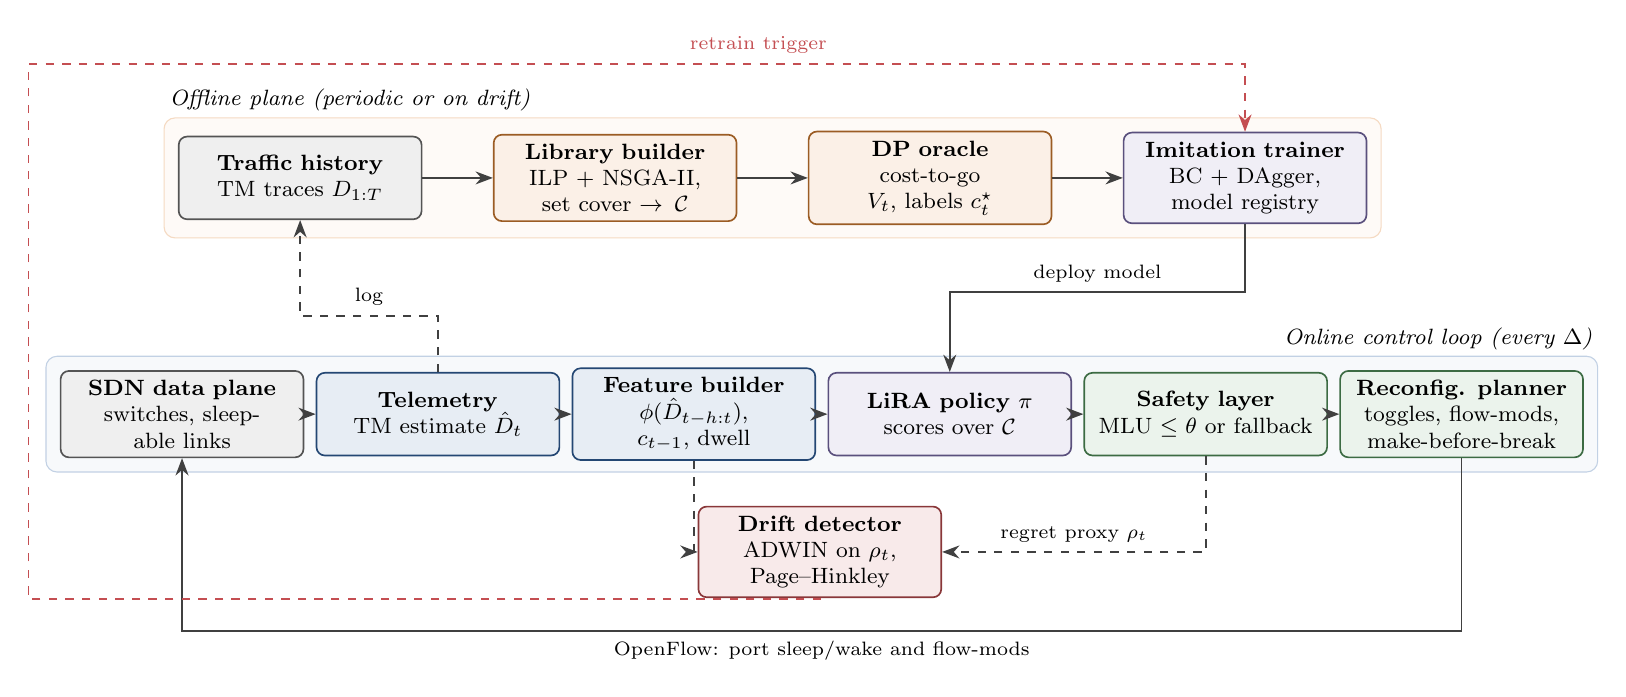
\begin{tikzpicture}[node distance=0.45cm]
\node[box=cGray] (hist) at (1.5,3.0) {\textbf{Traffic history}\\TM traces $D_{1:T}$};
\node[box=cOrange] (lib) at (5.5,3.0) {\textbf{Library builder}\\ILP + NSGA-II, set cover $\rightarrow\mathcal{C}$};
\node[box=cOrange] (dp) at (9.5,3.0) {\textbf{DP oracle}\\cost-to-go $V_t$, labels $c^\star_t$};
\node[box=cPurple] (train) at (13.5,3.0) {\textbf{Imitation trainer}\\BC + DAgger, model registry};
\node[box=cGray] (dpl) at (0,0) {\textbf{SDN data plane}\\switches, sleepable links};
\node[box] (tel) at (3.25,0) {\textbf{Telemetry}\\TM estimate $\hat{D}_t$};
\node[box] (feat) at (6.5,0) {\textbf{Feature builder}\\$\phi(\hat{D}_{t-h:t})$, $c_{t-1}$, dwell};
\node[box=cPurple] (pol) at (9.75,0) {\textbf{LiRA policy} $\pi$\\scores over $\mathcal{C}$};
\node[box=cGreen] (safe) at (13,0) {\textbf{Safety layer}\\$\mathrm{MLU}\le\theta$ or fallback};
\node[box=cGreen] (plan) at (16.25,0) {\textbf{Reconfig. planner}\\toggles, flow-mods, make-before-break};
\node[box=cRed] (drift) at (8.1,-1.75) {\textbf{Drift detector}\\ADWIN on $\rho_t$, Page--Hinkley};
\begin{scope}[on background layer]
\node[fill=cOrange!4,draw=cOrange!30,rounded corners=4pt,inner sep=5pt,fit=(hist)(train),label={[font=\footnotesize\itshape,anchor=south west,inner sep=2pt]north west:Offline plane (periodic or on drift)}] {};
\node[fill=cBlue!4,draw=cBlue!30,rounded corners=4pt,inner sep=5pt,fit=(dpl)(plan),label={[font=\footnotesize\itshape,anchor=south east,inner sep=2pt]north east:Online control loop (every $\Delta$)}] {};
\end{scope}
\draw[arr] (hist) -- (lib);
\draw[arr] (lib) -- (dp);
\draw[arr] (dp) -- (train);
\draw[arr] (dpl) -- (tel);
\draw[arr] (tel) -- (feat);
\draw[arr] (feat) -- (pol);
\draw[arr] (pol) -- (safe);
\draw[arr] (safe) -- (plan);
\draw[arr] (train.south) -- (13.5,1.55) -- node[above,font=\scriptsize,pos=0.5]{deploy model} (9.75,1.55) -- (pol.north);
\draw[darr] (tel.north) -- (3.25,1.25) -- node[above,font=\scriptsize]{log} (1.5,1.25) -- (hist.south);
\draw[arr] (plan.south) -- (16.25,-2.75) -- node[below,font=\scriptsize]{OpenFlow: port sleep/wake and flow-mods} (0,-2.75) -- (dpl.south);
\draw[darr] (feat.south) -- (6.5,-1.75) -- (drift.west);
\draw[darr] (safe.south) -- (13,-1.75) -- node[above,font=\scriptsize]{regret proxy $\rho_t$} (drift.east);
\draw[darr,draw=cRed] (drift.south) -- (8.1,-2.35) -- (-1.95,-2.35) -- (-1.95,4.45) -- node[above,font=\scriptsize,text=cRed,pos=0.6]{retrain trigger} (13.5,4.45) -- (train.north);
\end{tikzpicture}}
\caption{Architecture of LiRA. The offline plane builds the configuration library, computes sequence-optimal labels with the dynamic-programming oracle, and trains the policy. The online loop estimates the traffic matrix, selects a configuration conditioned on the installed one, enforces the utilization bound, and installs only the configuration difference. The drift detector triggers retraining.}
\label{fig:arch}
\end{figure*}

\subsection{Configuration Library}\label{sec:library}

The library must be small enough for fast decisions and rich enough to contain an efficient feasible configuration for almost every traffic matrix. We cluster training traffic matrices with $k$-medoids and, for each cluster, take both the medoid and the element-wise 95th-percentile matrix. For each representative matrix we solve the path-based energy-minimization ILP with $k=4$ shortest paths, link-pair sleeping, connectivity, and the utilization bound \eqref{eq:mlu}, and we run NSGA-II~\cite{deb2002nsga2} on power and maximum utilization to add Pareto-diverse link-state vectors. Duplicate vectors are merged, routing is re-optimized per vector by a linear program that minimizes maximum utilization, and a greedy set cover adds configurations until at least 99.5\% of training and validation matrices have a feasible member. The all-on configuration is always included. Finally, the library is pruned to $K$ configurations by greedy cost coverage, with $K=64$ by default.

\subsection{Exact Sequence-Optimal Oracle}

Because all terms of \eqref{eq:objective} depend only on $(c_{t-1},c_t,D_t)$, the problem is a shortest path through a trellis whose stages are intervals and whose states are library members (Fig.~\ref{fig:trellis}). Infeasible states receive infinite cost. The backward recursion \eqref{eq:dp} computes the cost-to-go $V_t(c)$ of being in configuration $c$ at the end of interval $t$, with $V_T\equiv 0$.
\begin{equation}\label{eq:dp}
\begin{aligned}V_{t-1}(c')&=\min_{c\in\mathcal{C}}Q_t(c',c),\\
Q_t(c',c)&=E(c,D_t)+\lambda_R R(c',c,D_t)\\
&\quad+\lambda_W W(c',c)+V_t(c)\end{aligned}
\end{equation}
The oracle trajectory follows $c^\star_t=\arg\min_c Q_t(c^\star_{t-1},c)$ from $c_0$. More importantly, the table $Q_t(c',\cdot)$ gives the optimal action for \emph{any} previously installed configuration $c'$, which we exploit for DAgger relabeling.

\begin{proposition}\label{prop:dp}
For a fixed library $\mathcal{C}$ and known $D_{1:T}$, recursion \eqref{eq:dp} returns a feasible sequence minimizing \eqref{eq:objective} whenever one exists, in $O(TK^2)$ time and $O(TK)$ memory.
\end{proposition}
\begin{IEEEproof}
By \eqref{eq:wear}, the wear contribution to $\overline{\mathrm{AF}}$ is a sum of terms that each depend on one pair of consecutive configurations, and \eqref{eq:energy} and \eqref{eq:reconf} depend on $(c_{t-1},c_t,D_t)$ only. Hence \eqref{eq:objective} is the length of a path from $c_0$ through a layered graph with $K$ nodes per layer, where the edge from $c'$ in layer $t-1$ to $c$ in layer $t$ has weight $E(c,D_t)+\lambda_R R(c',c,D_t)+\lambda_W W(c',c)$, and edges into infeasible nodes have infinite weight. Bellman's principle of optimality yields \eqref{eq:dp}, and each layer requires $K^2$ evaluations of precomputed quantities.
\end{IEEEproof}

\begin{figure}[t]
\centering
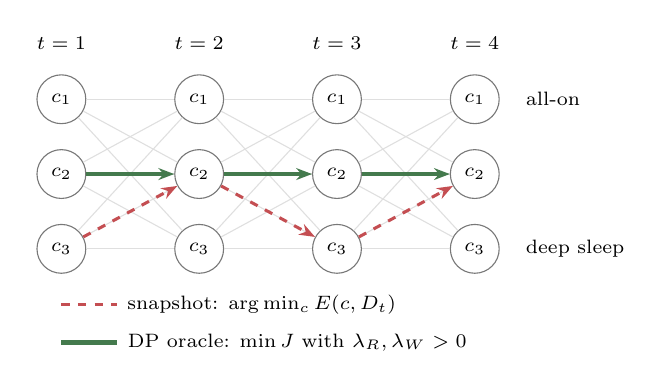
\begin{tikzpicture}[st/.style={circle,draw=cGray,fill=white,minimum size=0.62cm,inner sep=0pt,font=\scriptsize},x=1.75cm,y=0.95cm]
\foreach \t in {1,...,4}{\node[font=\scriptsize] at (\t,0.75) {$t=\t$};}
\foreach \t in {1,...,4}{\foreach \c/\y in {1/0,2/-1,3/-2}{\node[st] (n\t\c) at (\t,\y) {$c_{\c}$};}}
\foreach \t/\u in {1/2,2/3,3/4}{\foreach \a in {1,2,3}{\foreach \b in {1,2,3}{\draw[gray!25,line width=0.4pt] (n\t\a) -- (n\u\b);}}}
\draw[cRed,line width=1.1pt,dashed,-{Stealth[length=2mm]}] (n13) -- (n22);
\draw[cRed,line width=1.1pt,dashed,-{Stealth[length=2mm]}] (n22) -- (n33);
\draw[cRed,line width=1.1pt,dashed,-{Stealth[length=2mm]}] (n33) -- (n42);
\draw[cGreen!80!black,line width=1.6pt,-{Stealth[length=2mm]}] (n12) -- (n22);
\draw[cGreen!80!black,line width=1.6pt,-{Stealth[length=2mm]}] (n22) -- (n32);
\draw[cGreen!80!black,line width=1.6pt,-{Stealth[length=2mm]}] (n32) -- (n42);
\node[font=\scriptsize,anchor=west] at (4.3,0) {all-on};
\node[font=\scriptsize,anchor=west] at (4.3,-2) {deep sleep};
\draw[cRed,line width=1.1pt,dashed] (1.0,-2.75) -- (1.4,-2.75) node[right,font=\scriptsize,text=black] {snapshot: $\arg\min_c E(c,D_t)$};
\draw[cGreen!80!black,line width=1.6pt] (1.0,-3.25) -- (1.4,-3.25) node[right,font=\scriptsize,text=black] {DP oracle: $\min J$ with $\lambda_R,\lambda_W>0$};
\end{tikzpicture}
\caption{Configuration trellis. Nodes are library configurations per interval, and edges carry reconfiguration and wear costs. Snapshot selection flaps between $c_2$ and $c_3$ when traffic hovers near a decision boundary, whereas the oracle keeps $c_2$ because the extra energy is smaller than the switching cost.}
\label{fig:trellis}
\end{figure}

\subsection{History-Conditioned Policy}

The online policy $\pi_\vartheta(c\mid s_t)$ scores all $K$ configurations from the state in \eqref{eq:state}, where $\phi$ maps a traffic matrix to the log-scaled origin--destination vector, its total volume, the shares of the ten largest demands, and its principal components (95\% variance, fitted on training data), $\mathbf{1}_{c_{t-1}}$ is the one-hot encoding of the installed configuration, $\delta_{t-1}$ is its dwell time, and $\psi_t$ encodes time of day and day of week.
\begin{equation}\label{eq:state}
s_t=\big[\phi(\hat{D}_t),\phi(\hat{D}_{t-1}),\dots,\phi(\hat{D}_{t-h}),\mathbf{1}_{c_{t-1}},\delta_{t-1},\psi_t\big]
\end{equation}
We use gradient-boosted trees (LightGBM~\cite{ke2017lightgbm}) as the default model because the input is tabular and inference is fast. Section~\ref{sec:ablation} compares XGBoost~\cite{chen2016xgboost}, random forests~\cite{breiman2001rf}, a multilayer perceptron, and an LSTM~\cite{hochreiter1997lstm}.

\textbf{Regret-softened imitation.} Plain classification treats all mistakes as equal, although choosing a configuration that is almost as cheap as the optimum is harmless. We therefore train on soft targets derived from the oracle's action values, as in \eqref{eq:target}, and minimize the cross-entropy loss \eqref{eq:loss} over the training set $\mathcal{D}$, where $\beta>0$ is a temperature expressed in the same units as $J$. As $\beta\to 0$, the targets reduce to the oracle's hard labels.
\begin{equation}\label{eq:target}
q_t(c\mid c')=\frac{\exp\!\big(-(Q_t(c',c)-\min_{\tilde c}Q_t(c',\tilde c))/\beta\big)}{\sum_{\bar c}\exp\!\big(-(Q_t(c',\bar c)-\min_{\tilde c}Q_t(c',\tilde c))/\beta\big)}
\end{equation}
\begin{equation}\label{eq:loss}
\mathcal{L}(\vartheta)=-\sum_{(s_t,c')\in\mathcal{D}}\sum_{c\in\mathcal{C}}q_t(c\mid c')\log\pi_\vartheta(c\mid s_t)
\end{equation}

\textbf{DAgger.} A policy trained only on oracle trajectories never sees the states that its own mistakes create, and errors compound over time. We apply DAgger~\cite{ross2011dagger}: the current policy is rolled out on the training sequence, the visited pairs $(t,c_{t-1})$ are relabeled with $q_t(\cdot\mid c_{t-1})$ directly from the stored $Q$ tables without solving any new problem, and the policy is retrained on the aggregated data.

\subsection{Safety Layer}

At run time, the configuration with the highest score is checked against \eqref{eq:mlu} using $\hat{D}_t$. If it is infeasible, the controller falls back to the rule \eqref{eq:fallback}, which is evaluated for all $K$ configurations with one sparse matrix product.
\begin{equation}\label{eq:fallback}
c_t=\mathop{\arg\min}_{\substack{c\in\mathcal{C}\\\mathrm{MLU}(c,\hat{D}_t)\le\theta}}\Big[E(c,\hat{D}_t)+\lambda_R R(c_{t-1},c,\hat{D}_t)\Big]
\end{equation}
\begin{proposition}\label{prop:safety}
If the all-on configuration satisfies $\mathrm{MLU}\le\theta$ for $\hat{D}_t$, the safety layer always returns a configuration that satisfies \eqref{eq:mlu} for $\hat{D}_t$.
\end{proposition}
\begin{IEEEproof}
The all-on configuration belongs to $\mathcal{C}$ by construction, so the feasible set in \eqref{eq:fallback} is non-empty whenever the policy's choice is infeasible.
\end{IEEEproof}
The guarantee holds for the estimate $\hat{D}_t$. Violations with respect to the realized $D_t$ can still occur when traffic grows within an interval, and we report them as a metric.

\subsection{Drift Detection and Retraining}\label{sec:drift}

The oracle cannot be computed online, but a myopic regret proxy can. After each decision, the controller computes \eqref{eq:proxy}, which measures how much the chosen action loses against the best one-step action given the installed configuration, together with the indicator of a safety fallback.
\begin{equation}\label{eq:proxy}
\begin{split}\rho_t=\;&E(c_t,D_t)+\lambda_R R(c_{t-1},c_t,D_t)\\
&-\min_{c\in\mathcal{C}}\Big[E(c,D_t)+\lambda_R R(c_{t-1},c,D_t)\Big]\end{split}
\end{equation}
ADWIN~\cite{bifet2007adwin} monitors $\rho_t$ and the fallback rate, and a Page--Hinkley test~\cite{page1954cusum} monitors the total traffic volume and the first five principal components of $\phi(\hat{D}_t)$. When a detector fires, and at most once per 12-hour cooldown, the trainer recomputes oracle labels on a sliding window of the last $W$ days, warm-starts the model, and replaces it after validation on the most recent day. If more than 0.5\% of recent matrices have no feasible library member, new ILP solutions are added to the library.

\section{Algorithms}\label{sec:algorithms}

Algorithm~\ref{alg:offline} summarizes offline training and Algorithm~\ref{alg:online} the online control loop. Offline training is dominated by the library ILPs. By Proposition~\ref{prop:dp}, labeling costs $O(TK^2)$ per DAgger round, which takes seconds for a six-month Abilene trace with $K=64$. Online, each decision requires one model evaluation and at most one vectorized feasibility check over $K$ configurations.

\begin{algorithm}[t]
\caption{LiRA offline training}
\label{alg:offline}
\footnotesize
\begin{algorithmic}[1]
\Require training traces $D_{1:T}$, weights $\lambda_R,\lambda_W$, rounds $N$
\Ensure library $\mathcal{C}$, policy $\pi_\vartheta$
\State $\mathcal{C}\gets$ \Call{BuildLibrary}{$D_{1:T}$} \Comment{ILP, NSGA-II, set cover}
\State precompute $E(c,D_t)$, feasibility, $\|x-x'\|_1$, $\Delta F(c',c)$
\State compute $Q_t(c',c)$ and $V_t(c)$ by recursion \eqref{eq:dp}
\State $\mathcal{D}\gets\{(s_t,c^\star_{t-1})\}$ along the oracle trajectory
\State train $\pi_\vartheta$ on $\mathcal{D}$ with loss \eqref{eq:loss}
\For{$n=1$ to $N$}
\State roll out $\pi_\vartheta$ with safety layer, record $(t,c_{t-1})$
\State $\mathcal{D}\gets\mathcal{D}\cup\{(s_t,c_{t-1})\}$ with targets $q_t(\cdot\mid c_{t-1})$
\State retrain $\pi_\vartheta$ on $\mathcal{D}$; keep it if validation $J$ improves
\EndFor
\State \Return $\mathcal{C},\pi_\vartheta$
\end{algorithmic}
\end{algorithm}

\begin{algorithm}[t]
\caption{LiRA online control loop}
\label{alg:online}
\footnotesize
\begin{algorithmic}[1]
\Require $\mathcal{C}$, $\pi_\vartheta$, threshold $\theta$, initial $c_0$
\For{each interval $t=1,2,\dots$}
\State $\hat{D}_t\gets$ latest traffic-matrix estimate; build $s_t$ by \eqref{eq:state}
\State $c\gets\arg\max_{c}\pi_\vartheta(c\mid s_t)$
\If{$\mathrm{MLU}(c,\hat{D}_t)>\theta$}
\State $c\gets$ fallback rule \eqref{eq:fallback}
\EndIf
\If{$c\neq c_{t-1}$}
\State wake links in $x\setminus x_{t-1}$; install new rules (make-before-break)
\State remove stale rules; sleep links in $x_{t-1}\setminus x$
\EndIf
\State $c_t\gets c$; observe $D_t$; update detectors with $\rho_t$ from \eqref{eq:proxy}
\If{a detector fires and the cooldown has elapsed}
\State trigger Algorithm~\ref{alg:offline} on the last $W$ days (asynchronous)
\EndIf
\EndFor
\end{algorithmic}
\end{algorithm}

\section{Experimental Setup}\label{sec:setup}

\subsection{Datasets and Topologies}

Table~\ref{tab:datasets} lists the evaluation data. Abilene and G\'{E}ANT topologies and traffic matrices are taken from SNDlib~\cite{orlowski2010sndlib}, and the G\'{E}ANT matrices originate from~\cite{uhlig2006geant}. For Nobel-Germany, no multi-week measured trace was available to us, so we generate a 60-day semi-synthetic series by modulating the SNDlib demands with the diurnal and weekly profile and the residual noise distribution estimated from Abilene. For the scalability study, we use two large Topology Zoo graphs~\cite{knight2011zoo} with gravity-model traffic. Traffic is scaled so that the peak maximum link utilization under all-on shortest-path routing is 0.5. All splits are chronological (60\% training, 15\% validation, 25\% test), and scaling, principal components, and clustering are fitted on training data only.

\begin{table}[t]
\centering
\caption{Topologies and traffic data.}
\label{tab:datasets}
\footnotesize
\setlength{\tabcolsep}{3pt}
\begin{tabular}{@{}lccccc@{}}
\toprule
Topology & $|V|$ & $|E|$ & $\Delta$ & Span & Traffic \\
\midrule
Abilene & 12 & 15 & 5\,min & 24 weeks & real (SNDlib) \\
G\'{E}ANT & 22 & 36 & 15\,min & $\approx$4 months & real (SNDlib) \\
Nobel-Germany & 17 & 26 & 5\,min & 60 days & semi-synthetic \\
GtsCe (Zoo) & 149 & 193 & 5\,min & 7 days & gravity model \\
Cogent (Zoo) & 197 & 245 & 5\,min & 7 days & gravity model \\
\bottomrule
\end{tabular}
\end{table}

\subsection{Baselines}

We compare against: B0, all links always on with shortest-path routing, which is the energy reference; B1, the per-snapshot ILP solved on every test matrix; B2, a multi-period MILP that minimizes \eqref{eq:objective} over a rolling horizon of $H=12$ intervals with a persistence forecast; B3, NSGA-II per snapshot; B4, a snapshot classifier that maps each matrix to the library member defined by \eqref{eq:snapshot}, following~\cite{gomezdelahiz2025noms,gomezdelahiz2026tgcn} and using the same library, features, and safety layer as LiRA for fairness; B5, an ElasticTree-style greedy heuristic~\cite{heller2010elastictree}; B6, B4 with hysteresis, switching only if the predicted energy gain exceeds a tuned threshold; B7, B4 with a tuned minimum dwell time; and B8, PPO~\cite{schulman2017ppo} trained on the reward $-J$ per step. All tuning uses the validation split. We also report the offline oracle O$^\star$ as a lower bound.

\subsection{Metrics}

Energy savings $S$ are measured in port energy relative to B0. The retention $X=S_{\mathrm{LiRA}}/S_{\mathrm{B4}}$, the reduction in configuration changes $Y$, and the reduction in link power-state transitions $Z$ are computed relative to B4 per topology and averaged over the three topologies, as in \eqref{eq:metrics}.
\begin{equation}\label{eq:metrics}
X=\frac{S_{\mathrm{LiRA}}}{S_{\mathrm{B4}}},\quad Y=1-\frac{N^{\mathrm{ch}}_{\mathrm{LiRA}}}{N^{\mathrm{ch}}_{\mathrm{B4}}},\quad Z=1-\frac{N^{\mathrm{tr}}_{\mathrm{LiRA}}}{N^{\mathrm{tr}}_{\mathrm{B4}}}
\end{equation}
We also report the total cost $J$ normalized to B4, the regret against O$^\star$, the percentage of intervals with realized MLU above $\theta$, the mean acceleration factor $\overline{\mathrm{AF}}$ from \eqref{eq:af}, and the median and 99th-percentile decision latency measured single-threaded with batch size one over $10^4$ decisions.

\subsection{Implementation and Parameters}

The flow-level simulator is written in Python with NumPy and sparse path--link matrices. ILPs are solved with Gurobi~11~\cite{gurobi} (MIP gap 1\%, 300\,s limit), with HiGHS~\cite{huangfu2018highs} as an open-source check. NSGA-II uses pymoo, the drift detectors use the river library, and PPO uses Stable-Baselines3. Experiments run on a server with two Intel Xeon Gold 6338 CPUs, 256\,GB of RAM, and one NVIDIA A100 GPU, used only for the neural baselines. Emulation uses Mininet~2.3~\cite{lantz2010mininet} with Open vSwitch and the Ryu controller~\cite{ryu} in an Ubuntu 22.04 virtual machine with 16 vCPUs. Table~\ref{tab:params} lists the parameters. Hyperparameters were selected with 50 Optuna trials per model on validation $J$ for LiRA and on validation macro-F1 for B4. Stochastic components use five seeds, and results report means with 95\% bootstrap confidence intervals. Code, configuration files, data-preparation scripts, and per-interval decision logs will be released with the paper, and an anonymized repository is available to reviewers.

\begin{table}[t]
\centering
\caption{Model and training parameters.}
\label{tab:params}
\footnotesize
\setlength{\tabcolsep}{3pt}
\begin{tabular}{@{}p{4.75cm}p{3.75cm}@{}}
\toprule
Parameter & Value \\
\midrule
Utilization threshold $\theta$; paths $k$; library $K$ & 0.8; 4; 64 \\
Port-pair power $P^{\mathrm{idle}}$/$P^{\mathrm{dyn}}$/$P^{\mathrm{sl}}$ & 30/5/3\,W \\
Wear model $\alpha^{\mathrm{off}}$; $\chi$ & 0.5; 0.6\,h \\
Price of one change; one transition & 0.2\%; 0.08\% of daily B0 energy \\
History $h$; DAgger rounds $N$; $\beta$ & 3; 4; 0.05 \\
LightGBM leaves / rate / trees & 63 / 0.05 / 800 \\
LightGBM feature / bagging fraction & 0.8 / 0.8 \\
MLP baseline & 2$\times$256 ReLU, Adam $10^{-3}$, batch 512 \\
PPO & lr $3\cdot10^{-4}$, $\gamma=0.99$, $2\cdot10^{6}$ steps \\
ADWIN $\delta$; cooldown; window $W$ & 0.002; 12\,h; 7 days \\
\bottomrule
\end{tabular}
\end{table}

\subsection{Experimental Pipeline}

Fig.~\ref{fig:pipeline} shows the pipeline. Every method produces a per-interval configuration log in a common format, and all metrics are computed from these logs by the same evaluation code. Mininet emulation replays a 24-hour segment of the Abilene test period for B4, B6, and LiRA, with link capacities scaled by $1/100$, one interval compressed to 30\,s, and a modeled link wake-up delay of 1\,s before a port carries traffic.

\begin{figure}[t]
\centering
\resizebox{\columnwidth}{!}{%
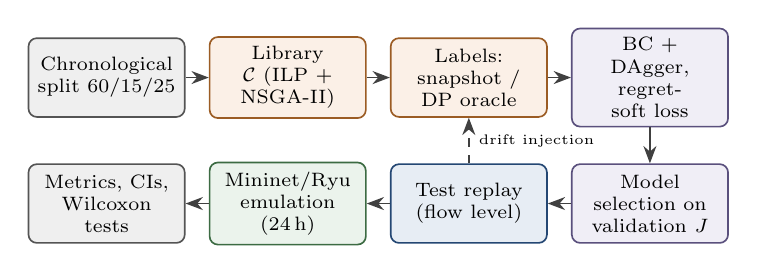
\begin{tikzpicture}[pb/.style={box=#1,text width=1.75cm,minimum height=1.0cm,font=\scriptsize}]
\node[pb=cGray] (a) at (0,0) {Chronological split 60/15/25};
\node[pb=cOrange] (b) at (2.3,0) {Library $\mathcal{C}$ (ILP + NSGA-II)};
\node[pb=cOrange] (c) at (4.6,0) {Labels: snapshot / DP oracle};
\node[pb=cPurple] (d) at (6.9,0) {BC + DAgger, regret-soft loss};
\node[pb=cPurple] (e) at (6.9,-1.6) {Model selection on validation $J$};
\node[pb=cBlue] (f) at (4.6,-1.6) {Test replay (flow level)};
\node[pb=cGreen] (g) at (2.3,-1.6) {Mininet/Ryu emulation (24\,h)};
\node[pb=cGray] (h) at (0,-1.6) {Metrics, CIs, Wilcoxon tests};
\draw[arr] (a) -- (b);
\draw[arr] (b) -- (c);
\draw[arr] (c) -- (d);
\draw[arr] (d) -- (e);
\draw[arr] (e) -- (f);
\draw[arr] (f) -- (g);
\draw[arr] (g) -- (h);
\draw[darr] (f.north) -- (c.south) node[midway,right,font=\tiny]{drift injection};
\end{tikzpicture}}
\caption{Training and evaluation pipeline. All methods share the split, the library, and the evaluation code, and only the decision rule differs.}
\label{fig:pipeline}
\end{figure}

\section{Results and Discussion}\label{sec:results}

\subsection{Energy Versus Stability}

Table~\ref{tab:main} reports the main comparison. The per-snapshot ILP (B1) attains the highest savings, between 38.2\% and 44.7\%, but it also changes configuration most often after the genetic algorithm and needs seconds to tens of seconds per decision. The snapshot classifier (B4) recovers most of these savings in about one millisecond, which confirms the premise of learned configuration, but it changes configuration 27.3 to 61.4 times per day. LiRA retains 94.6\%, 94.9\%, and 94.7\% of the B4 savings on Abilene, G\'{E}ANT, and Nobel-Germany, while reducing configuration changes by 76.7\%, 75.1\%, and 76.5\% and link power-state transitions by 79.2\%, 81.7\%, and 79.1\%. Averaged over the three topologies, this yields $X=\resRetention\%$ (CI$_{95\%}$=[93.9, 95.4]), $Y=\resChangeRed\%$, and $Z=\resTransRed\%$. Transitions fall more than configuration changes because LiRA prefers transitions between configurations that differ in few links, which the reconfiguration term rewards.

\begin{table*}[t]
\centering
\caption{Main results on the test periods: port-energy savings $S$ relative to always-on (\%), configuration changes per day (Ch.), link power-state transitions per day (Tr.), and median decision latency on G\'{E}ANT. 95\% CI half-widths are below 0.6 percentage points for $S$ and below 8\% of the mean for Ch. and Tr.}
\label{tab:main}
\footnotesize
\setlength{\tabcolsep}{4.5pt}
\begin{tabular}{@{}llccccccccccc@{}}
\toprule
& & \multicolumn{3}{c}{Abilene} & \multicolumn{3}{c}{G\'{E}ANT} & \multicolumn{3}{c}{Nobel-Germany} & \\
\cmidrule(lr){3-5}\cmidrule(lr){6-8}\cmidrule(lr){9-11}
ID & Method & $S$ (\%) & Ch. & Tr. & $S$ (\%) & Ch. & Tr. & $S$ (\%) & Ch. & Tr. & Latency \\
\midrule
B1 & Per-snapshot ILP & 38.2 & 74.2 & 251.0 & 44.7 & 33.5 & 158.2 & 41.3 & 66.1 & 230.5 & 38.5\,s \\
B2 & Multi-period MILP ($H=12$) & 35.1 & 10.6 & 39.8 & 41.2 & 5.6 & 23.0 & 38.0 & 9.7 & 36.1 & 412\,s \\
B3 & NSGA-II per snapshot & 35.1 & 88.6 & 302.4 & 40.2 & 39.1 & 189.7 & 37.6 & 79.3 & 271.8 & 31.4\,s \\
B4 & Snapshot ML & 36.9 & 61.4 & 214.6 & 43.1 & 27.3 & 131.8 & 39.8 & 54.8 & 197.3 & 1.4\,ms \\
B5 & ElasticTree-style greedy & 29.4 & 47.3 & 96.8 & 33.0 & 21.6 & 58.4 & 31.2 & 42.5 & 88.1 & 112\,ms \\
B6 & B4 + hysteresis & 34.0 & 22.7 & 81.5 & 40.1 & 10.8 & 50.3 & 36.9 & 20.5 & 74.6 & 1.5\,ms \\
B7 & B4 + minimum dwell & 33.1 & 18.9 & 69.0 & 39.0 & 9.6 & 44.1 & 35.8 & 17.2 & 63.2 & 1.4\,ms \\
B8 & PPO & 32.8 & 15.6 & 58.2 & 37.9 & 7.9 & 36.4 & 35.0 & 14.1 & 52.7 & 1.0\,ms \\
\midrule
-- & \textbf{LiRA} & \textbf{34.9} & \textbf{14.3} & \textbf{44.7} & \textbf{40.9} & \textbf{6.8} & \textbf{24.1} & \textbf{37.7} & \textbf{12.9} & \textbf{41.2} & \textbf{2.3\,ms} \\
O$^\star$ & Offline oracle & 35.8 & 11.2 & 39.5 & 42.0 & 5.3 & 21.8 & 38.9 & 10.1 & 36.0 & offline \\
\bottomrule
\end{tabular}
\end{table*}

Fig.~\ref{fig:pareto} places these results on the energy--stability plane for Abilene by sweeping $\lambda_R$ for LiRA and O$^\star$, the threshold for B6, and the dwell time for B7. For every number of changes per day, LiRA saves more energy than both heuristics, and it stays within 0.6 to 2.2 percentage points of the oracle frontier, with the largest gap at the most conservative setting. Hysteresis and minimum dwell suppress changes uniformly, whereas LiRA suppresses only the changes whose energy gain does not justify their cost.

\begin{figure}[t]
\centering
\begin{tikzpicture}
\begin{axis}[width=\columnwidth,height=5.0cm,xlabel={Configuration changes per day},ylabel={Energy savings $S$ (\%)},xmin=0,xmax=80,ymin=26.5,ymax=39,legend pos=south east,legend columns=2]
\addplot[cBlue,thick,mark=*,mark size=1.6pt] table[x=changes,y=savings]{data/pareto_lira.dat};
\addlegendentry{LiRA}
\addplot[black,dashed,mark=o,mark size=1.6pt] table[x=changes,y=savings]{data/pareto_oracle.dat};
\addlegendentry{Oracle O$^\star$}
\addplot[cOrange,thick,mark=square*,mark size=1.4pt] table[x=changes,y=savings]{data/pareto_hyst.dat};
\addlegendentry{B6 hysteresis}
\addplot[cGreen,thick,mark=triangle*,mark size=1.8pt] table[x=changes,y=savings]{data/pareto_dwell.dat};
\addlegendentry{B7 min. dwell}
\addplot[cRed,only marks,mark=star,mark size=3pt,thick] table[x=changes,y=savings]{data/pareto_snap.dat};
\addlegendentry{B4 snapshot}
\addplot[cPurple,only marks,mark=diamond*,mark size=2.4pt] table[x=changes,y=savings]{data/pareto_ilp.dat};
\addlegendentry{B1 ILP}
\end{axis}
\end{tikzpicture}
\caption{Energy--stability trade-off on Abilene. LiRA and the oracle are swept over $\lambda_R$, B6 over its hysteresis threshold, and B7 over its dwell time. Points further up and to the left are better.}
\label{fig:pareto}
\end{figure}

\subsection{Behavior Over Time}

Fig.~\ref{fig:timeseries} shows the number of active links over one test day on Abilene. Both methods follow the diurnal pattern, putting up to eight links to sleep at night. B4 flaps between adjacent levels whenever demand hovers near a decision boundary, producing 60 changes on this day, whereas LiRA produces 14 changes and holds a slightly larger active set ahead of the morning ramp, because waking a link later costs a transition.

\begin{figure}[t]
\centering
\begin{tikzpicture}
\begin{axis}[width=\columnwidth,height=4.6cm,xlabel={Hour of day},ylabel={Active links},xmin=0,xmax=24,ymin=0,ymax=16.5,xtick={0,4,...,24},legend style={at={(0.5,1.03)},anchor=south},legend columns=3]
\addplot[fill=gray!18,draw=none] table[x=hour,y=traffic]{data/timeseries.dat} \closedcycle;
\addlegendentry{traffic (scaled)}
\addplot[cRed,const plot,line width=0.5pt] table[x=hour,y=snap]{data/timeseries.dat};
\addlegendentry{B4}
\addplot[cBlue,const plot,line width=1.2pt] table[x=hour,y=lira]{data/timeseries.dat};
\addlegendentry{LiRA}
\end{axis}
\end{tikzpicture}
\caption{Active links over one Abilene test day (5-minute intervals). B4 changes configuration 60 times and LiRA 14 times on this day.}
\label{fig:timeseries}
\end{figure}

\subsection{Total Cost, Feasibility, and Lifetime}

Table~\ref{tab:cost} aggregates total cost, regret, feasibility, and wear over the three topologies. LiRA lowers the total cost $J$ by 19.6\% relative to B4 and is within 2.9\% of the oracle. Only the multi-period MILP (B2) is closer to the oracle, at 1.2\%, but it needs several minutes per decision and violates the utilization bound more often because its forecast errors are not covered by a safety layer. PPO reaches a comparable number of changes but violates the bound in 1.14\% of intervals, five times more often than LiRA. Wilcoxon signed-rank tests on daily cost (42, 30, and 15 test days) reject equality between LiRA and each of B4, B6, and B7 on every topology after Holm correction ($p<0.001$ on Abilene and G\'{E}ANT and $p<0.01$ on Nobel-Germany), with Cliff's $\delta$ between 0.71 and 0.94.

\begin{table}[t]
\centering
\caption{Averages over the three topologies: total cost relative to B4, regret against the oracle, intervals with realized MLU above $\theta$, and mean acceleration factor (always-on: 1.000).}
\label{tab:cost}
\footnotesize
\setlength{\tabcolsep}{4pt}
\begin{tabular}{@{}lcccc@{}}
\toprule
Method & $J/J_{\mathrm{B4}}$ & Regret (\%) & MLU viol. (\%) & $\overline{\mathrm{AF}}$ \\
\midrule
B1 Per-snapshot ILP & 1.036 & 32.9 & 0.00 & 1.020 \\
B2 Multi-period MILP & 0.791 & 1.2 & 0.48 & 0.827 \\
B3 NSGA-II & 1.147 & 47.1 & 0.00 & 1.090 \\
B4 Snapshot ML & 1.000 & 28.2 & 0.27 & 0.991 \\
B5 Greedy & 0.987 & 26.3 & 0.00 & 0.922 \\
B6 Hysteresis & 0.860 & 10.1 & 0.34 & 0.875 \\
B7 Minimum dwell & 0.857 & 9.6 & 0.45 & 0.869 \\
B8 PPO & 0.851 & 8.8 & 1.14 & 0.862 \\
\midrule
\textbf{LiRA} & \textbf{0.804} & \textbf{2.9} & \textbf{0.23} & \textbf{0.833} \\
O$^\star$ & 0.782 & 0.0 & 0.00 & 0.822 \\
\bottomrule
\end{tabular}
\end{table}

Fig.~\ref{fig:af} breaks the acceleration factor down by topology. On Abilene, the frequent transitions of B1 and B4 push the factor above one, so the snapshot methods would age line cards faster than an always-on network despite saving energy. This is the effect that motivates the title. LiRA lowers the factor to 0.881 on Abilene, 0.790 on G\'{E}ANT, and 0.830 on Nobel-Germany. G\'{E}ANT is less affected because its 15-minute intervals offer fewer opportunities to flap.

\begin{figure}[t]
\centering
\begin{tikzpicture}
\begin{axis}[width=\columnwidth,height=4.6cm,ybar,bar width=4.2pt,ymin=0.7,ymax=1.25,ylabel={Mean acceleration factor},xtick=data,xticklabels from table={data/af.dat}{method},x tick label style={font=\scriptsize},enlarge x limits=0.1,legend style={at={(0.5,1.03)},anchor=south},legend columns=3]
\addplot[fill=cBlue!70,draw=cBlue] table[x expr=\coordindex,y=abilene]{data/af.dat};
\addlegendentry{Abilene}
\addplot[fill=cOrange!70,draw=cOrange] table[x expr=\coordindex,y=geant]{data/af.dat};
\addlegendentry{G\'{E}ANT}
\addplot[fill=cGreen!70,draw=cGreen] table[x expr=\coordindex,y=nobel]{data/af.dat};
\addlegendentry{Nobel}
\draw[cRed,dashed,thick] (axis cs:-0.6,1) -- (axis cs:5.6,1);
\end{axis}
\end{tikzpicture}
\caption{Mean failure-rate acceleration factor from \eqref{eq:af} per method and topology. The dashed line marks the always-on network. Values above it mean faster ageing than without sleep modes.}
\label{fig:af}
\end{figure}

\subsection{Decision Latency and Scalability}

Fig.~\ref{fig:latency} reports the median decision latency as a function of topology size. LiRA takes 1.8 to 2.3\,ms on the three evaluation topologies, including the feasibility check, with 99th percentiles of 3.9 to 4.6\,ms, and 7.4\,ms on the 245-link Cogent graph. Its overhead over B4 comes from the history features and from the safety check, which runs on every decision. The ILP and NSGA-II reach the 300\,s limit on the Topology Zoo graphs, where the ILP terminates with an average MIP gap of 4.7\%. Training LiRA, including library construction, takes 3.1\,h on G\'{E}ANT, of which 92\% is spent in library ILPs, whereas oracle labeling for four DAgger rounds takes 41\,s.

\begin{figure}[t]
\centering
\begin{tikzpicture}
\begin{axis}[width=\columnwidth,height=4.6cm,xmode=log,ymode=log,xlabel={Number of links $|E|$},ylabel={Median decision time (ms)},xmin=12,xmax=300,ymin=0.5,ymax=1e6,xtick={15,26,36,193,245},xticklabels={15,26,36,193,245},legend style={at={(0.5,1.03)},anchor=south},legend columns=3]
\addplot[cBlue,thick,mark=*,mark size=1.5pt] table[x=links,y=lira]{data/latency.dat};
\addlegendentry{LiRA}
\addplot[cRed,thick,mark=star,mark size=2pt] table[x=links,y=snap]{data/latency.dat};
\addlegendentry{B4 snapshot}
\addplot[cGreen,thick,mark=triangle*,mark size=1.6pt] table[x=links,y=greedy]{data/latency.dat};
\addlegendentry{B5 greedy}
\addplot[cOrange,thick,mark=square*,mark size=1.3pt] table[x=links,y=ga]{data/latency.dat};
\addlegendentry{B3 NSGA-II}
\addplot[cPurple,thick,mark=diamond*,mark size=1.8pt] table[x=links,y=ilp]{data/latency.dat};
\addlegendentry{B1 ILP}
\draw[gray,dashed] (axis cs:12,3e5) -- (axis cs:300,3e5) node[pos=0.97,below,font=\scriptsize,anchor=north east]{300\,s limit};
\end{axis}
\end{tikzpicture}
\caption{Median decision time versus topology size (Abilene, Nobel-Germany, G\'{E}ANT, GtsCe, Cogent). Solver-based methods hit the 300\,s limit on the large graphs.}
\label{fig:latency}
\end{figure}

\subsection{Ablation Study}\label{sec:ablation}

Table~\ref{tab:ablation} removes one component at a time on Abilene. Removing the installed configuration from the input has the largest effect: the model then cannot distinguish staying from switching and changes configuration 52.6 times per day, close to B4, which shows that the oracle labels alone do not produce stability. Without DAgger, compounding errors raise the number of changes by 50\%. Traffic history and the regret-softened loss each contribute between 2\% and 4\% of total cost. Removing the safety layer barely changes energy and stability but raises utilization violations from 0.18\% to 1.62\%. Setting $\lambda_W=0$ keeps the number of changes but increases transitions by 20\%, because the policy no longer prefers configurations that differ in few links. Among the model families, XGBoost is within 0.4\% of LightGBM in total cost, random forests are 3.2\% worse, the multilayer perceptron is 1.9\% worse, and the LSTM is 1.1\% worse at 3.4 times the latency. Varying the library size on G\'{E}ANT, LiRA saves 31.2\%, 37.4\%, 39.8\%, 40.9\%, 41.2\%, and 41.3\% for $K=8$, 16, 32, 64, 128, and 256, while median latency grows from 1.2\,ms to 5.8\,ms, which motivates $K=64$.

\begin{table}[t]
\centering
\caption{Ablation on Abilene (test period).}
\label{tab:ablation}
\footnotesize
\setlength{\tabcolsep}{3.5pt}
\begin{tabular}{@{}lccccc@{}}
\toprule
Variant & $S$ (\%) & Ch. & Tr. & Viol. (\%) & $J/J_{\mathrm{B4}}$ \\
\midrule
\textbf{LiRA (full)} & \textbf{34.9} & \textbf{14.3} & \textbf{44.7} & \textbf{0.18} & \textbf{0.773} \\
-- installed config.\ input & 36.4 & 52.6 & 181.3 & 0.20 & 0.958 \\
-- traffic history ($h=0$) & 34.6 & 19.6 & 62.5 & 0.19 & 0.803 \\
-- regret-softened loss & 34.3 & 16.8 & 54.0 & 0.18 & 0.793 \\
-- DAgger & 33.7 & 21.5 & 69.9 & 0.24 & 0.823 \\
-- safety layer & 35.2 & 14.1 & 44.0 & 1.62 & 0.769 \\
$\lambda_W=0$ & 35.1 & 14.0 & 53.6 & 0.18 & 0.778 \\
\bottomrule
\end{tabular}
\end{table}

\subsection{Robustness to Traffic Drift}

We inject five shifts into the Abilene test period and compare no retraining, daily periodic retraining, and drift-triggered retraining. Table~\ref{tab:drift} reports the ADWIN detection delay and the excess cost over the oracle during the seven days after each shift. Without retraining, the excess cost rises to between 9.6\% and 22.4\%. Triggered retraining keeps it between 2.2\% and 4.1\%, which is comparable to daily retraining while using 6 retraining runs over the six-week test period instead of 42. For the permanent link failure, triggered retraining outperforms daily retraining because it reacts within minutes. The false-alarm rate on unmodified test data is 0.41 per 1000 intervals. Fig.~\ref{fig:drift} shows the trajectory for the sudden volume step. Weekly retraining recovers only at its next scheduled run, whereas triggered retraining recovers within about one day as post-drift data accumulates in the training window.

\begin{table}[t]
\centering
\caption{Drift scenarios on Abilene: ADWIN detection delay and excess cost over the oracle (\%) during the seven days after the shift.}
\label{tab:drift}
\footnotesize
\setlength{\tabcolsep}{3pt}
\begin{tabular}{@{}lcccc@{}}
\toprule
Scenario & Delay & No retrain & Daily & Triggered \\
\midrule
Volume step $+40\%$ & 35\,min & 18.7 & 2.6 & 3.1 \\
Growth ramp $+60\%$ in 7 days & 305\,min & 11.2 & 2.0 & 2.4 \\
Diurnal phase shift 6\,h & 70\,min & 9.6 & 2.9 & 2.2 \\
Hotspot (top pair $\times3$) & 45\,min & 14.3 & 3.0 & 3.5 \\
Permanent link failure & 15\,min & 22.4 & 5.8 & 4.1 \\
\midrule
Retraining runs (6 weeks) & -- & 0 & 42 & 6 \\
\bottomrule
\end{tabular}
\end{table}

\begin{figure}[t]
\centering
\begin{tikzpicture}
\begin{axis}[width=\columnwidth,height=4.4cm,xlabel={Day of test period},ylabel={Excess cost over O$^\star$ (\%)},xmin=0,xmax=14,ymin=0,ymax=24,xtick={0,2,...,14},legend style={at={(0.5,1.03)},anchor=south},legend columns=3]
\addplot[cRed,line width=0.5pt] table[x=day,y=none]{data/drift.dat};
\addlegendentry{no retrain}
\addplot[cOrange,line width=0.6pt] table[x=day,y=weekly]{data/drift.dat};
\addlegendentry{weekly}
\addplot[cBlue,line width=0.9pt] table[x=day,y=triggered]{data/drift.dat};
\addlegendentry{triggered}
\draw[black,dashed] (axis cs:5,0) -- (axis cs:5,24) node[pos=0.55,left,font=\scriptsize]{drift};
\draw[cOrange,dotted,thick] (axis cs:7,0) -- (axis cs:7,24);
\end{axis}
\end{tikzpicture}
\caption{Hourly excess cost after a sudden $+40\%$ volume step at day 5 on Abilene. The dotted line marks the next weekly retraining.}
\label{fig:drift}
\end{figure}

\subsection{Emulation of Transition Effects}

Table~\ref{tab:emu} reports the Mininet replay. Because LiRA changes configuration less often and prefers small differences, it sends 78\% fewer flow-modification messages than B4. Each reconfiguration also installs faster, in 12.6\,ms versus 18.4\,ms at the median, because fewer rules change per update. Aggregate packet loss drops from 0.112\% to 0.029\%, and the 99th-percentile round-trip time from 41.7\,ms to 19.8\,ms. These effects are invisible in flow-level evaluations and add to the case for stability.

\begin{table}[t]
\centering
\caption{Mininet/Ryu replay of a 24-hour Abilene segment (mean of five runs; standard deviation below 6\% of the mean).}
\label{tab:emu}
\footnotesize
\setlength{\tabcolsep}{4pt}
\begin{tabular}{@{}lccc@{}}
\toprule
Metric & B4 & B6 & LiRA \\
\midrule
Configuration changes & 61 & 23 & 14 \\
Flow-mod messages & 3912 & 1401 & 862 \\
Median reconfiguration time (ms) & 18.4 & 17.9 & 12.6 \\
Packet loss (\%) & 0.112 & 0.047 & 0.029 \\
99th-percentile RTT (ms) & 41.7 & 26.3 & 19.8 \\
Controller CPU (\%) & 7.9 & 4.1 & 3.2 \\
\bottomrule
\end{tabular}
\end{table}

\section{Comparative Analysis}\label{sec:comparison}

The results separate the methods into three groups. Solver-based methods (B1, B3) maximize per-interval savings but are too slow for five-minute control on large graphs and are the least stable, because exact per-snapshot optima jump between near-equivalent configurations. The multi-period MILP (B2) shows that optimizing the sequence pays off, since it is the closest method to the oracle in total cost, but its run time of minutes per decision and its forecast-induced violations prevent online use. Learned snapshot methods (B4) and their heuristic fixes (B6, B7) are fast, but the fixes trade energy for stability with a single global knob, which is why they lie below LiRA in Fig.~\ref{fig:pareto}. LiRA combines the decision speed of B4 with most of the sequence-level benefit of B2, and its gap to the oracle (2.9\%) is smaller than that of any other online method. Compared with PPO, imitating an exact oracle needs no reward shaping or exploration and gives five times fewer utilization violations, because the oracle labels are feasible by construction and the safety layer covers the remaining cases. The practical implication is that operators adopting learned energy-aware configuration should price reconfiguration and wear explicitly. Doing so costs about five percent of the snapshot energy savings and removes three quarters of the configuration churn.

Deployment requires little beyond what snapshot frameworks already assume. The controller needs a traffic-matrix estimate per interval, a southbound interface that can put ports to sleep, and the library computed offline. The prices $\lambda_R$ and $\lambda_W$ are operator policy rather than model parameters: they can be set from the expected cost of a maintenance event and the operator's tolerance for update traffic, and Fig.~\ref{fig:pareto} shows the savings that each setting gives up. Because the safety layer and the all-on fallback are independent of the model (Proposition~\ref{prop:safety}), a mispredicting model degrades to higher energy use rather than to congestion.

\section{Limitations}\label{sec:limitations}

Several limitations qualify these findings. First, the wear model \eqref{eq:af} is a normalized linear abstraction of~\cite{chiaraviglio2015lifetime} with assumed parameters, so absolute lifetime figures should not be read as predictions for specific hardware. For this reason we also report raw transition counts, which do not depend on the model. Second, the port power values are representative rather than measured on a particular router, and savings scale with the share of power that sleep can remove. Third, the Nobel-Germany trace is semi-synthetic, and the large topologies use gravity-model traffic, so real-trace conclusions rest on Abilene and G\'{E}ANT. Fourth, LiRA is limited by its library. A traffic regime that no library member serves efficiently requires a library refresh, which is triggered by the fallback rate but takes hours of ILP time. Fifth, Mininet does not reproduce line-card wake-up physics, which we approximate by a fixed delay. Finally, the safety guarantee applies to the estimated traffic matrix and does not cover traffic growth within an interval.

\section{Conclusion and Future Work}\label{sec:conclusion}

We showed that learned energy-aware SDN configuration should be treated as a sequence of decisions. Over a finite configuration library, energy, reconfiguration, and the mean wear acceleration factor combine into an objective that dynamic programming minimizes exactly, and a history-conditioned policy trained by imitation of this oracle approaches it online in about two milliseconds. On Abilene, G\'{E}ANT, and Nobel-Germany, LiRA retained \resRetention\% of the energy savings of a snapshot classifier while reducing configuration changes by \resChangeRed\% and link power-state transitions by \resTransRed\%, kept the modeled acceleration factor below that of an always-on network, and recovered from traffic drift with few retraining runs. Future work will calibrate the wear model with field failure data, learn the library jointly with the policy, extend the formulation to adaptive link rate and multi-domain settings, and evaluate LiRA on a hardware testbed with real sleep-capable line cards.

\bibliographystyle{IEEEtran}
\bibliography{references}

\end{document}
